

\documentclass{article}
%\usepackage[margin=1in]{geometry}
\setlength\topmargin{0pt}
\addtolength\topmargin{-\headheight}
\addtolength\topmargin{-\headsep}
\setlength\oddsidemargin{0pt}
\setlength\textwidth{\paperwidth}
\addtolength\textwidth{-2in}
\setlength\textheight{\paperheight}
\addtolength\textheight{-2in}

\usepackage[english]{babel}
\usepackage[utf8]{inputenc}
\usepackage{fancyhdr}
\usepackage{listings}
\usepackage{graphicx}
\usepackage{xcolor}


\definecolor{codegreen}{rgb}{0,0.6,0}
\definecolor{codegray}{rgb}{0.5,0.5,0.5}
\definecolor{codepurple}{rgb}{0.58,0,0.82}
\definecolor{backcolour}{rgb}{0.95,0.95,0.92}


\usepackage{booktabs}
\usepackage{pgfplotstable}



\lstdefinestyle{mystyle}{
	backgroundcolor=\color{backcolour},   
	commentstyle=\color{codegreen},
	keywordstyle=\color{magenta},
	numberstyle=\tiny\color{codegray},
	stringstyle=\color{codepurple},
	basicstyle=\ttfamily\footnotesize,
	breakatwhitespace=false,         
	breaklines=true,                 
	captionpos=b,                    
	keepspaces=true,                 
	numbers=left,                    
	numbersep=5pt,                  
	showspaces=false,                
	showstringspaces=false,
	showtabs=false,                  
	tabsize=2
}
\lstset{style=mystyle}


% header
\pagestyle{fancy}
\fancyhf{}
\rhead{CS 491}
\lhead{Pedram Safaei and Kevin Carlos}
\rfoot{Page \thepage}
\usepackage{listings}

\begin{document}
	\section{Nearest Neighbor}
	\subsection{Describe Implementation}
	The general idea is to compute the L2 Norm to the nearest neighbor, K point, and return the most recurring label in those neighbors.
	
	\subsubsection{KNN\_TEST}
	This function genrates a label based on the points given to it, computes the distance, to each of those points (training points) and puts them in a list. This list is then sorted based on the distance that was calculated before. The subset of the K nearest neighbor or point will have their labels summed and then we will output the sign of the summation as the label, so if our predicted label is less than 0 we return -1 and if it is greater than 0 we return 1. In case the predicted value is 0 we will choose the result based on the ordering of the training data and from the set of neighbors in the sorted list.
	\begin{lstlisting}[language=Python]
	def KNN_test(X_train, Y_train, X_test, Y_test,K):
		NumberOfCorrect = 0
		for i, j in enumerate(X_test):
			radius = []
			for n, m in enumerate(X_train):
				radius.append(((math.pow((m[0] - j[0]), 2) + math.pow((m[1] - j[1]), 2)), Y_train[n][0]))
		List_sorted = sorted(radius, key=lambda member: member[0], reverse=False)[:K] 
		predictedvalue = sum([member[1] for member in List_sorted])
		if (not predictedvalue):
			predictedvalue = List_sorted[0][1]
		elif (predictedvalue < 0):
			predictedvalue = -1
		elif (predictedvalue > 0):
			predictedvalue = 1
		if predictedvalue == Y_test[i][0]:
			NumberOfCorrect = NumberOfCorrect+1
		return NumberOfCorrect / len(X_test)
	\end{lstlisting}
	
	\subsubsection{Choose\_K}
	This function is simply checking all possible accuracies on the given test data and returns the index with the greatest accuracy which will be our K.
	\begin{lstlisting}[language=Python]
		OldAccuracy = 0
		NewAccuracy = 0
		Predicted_K = 1
		K = len(X_train)
		for i in range(1, K):
			OldAccuracy = KNN_test(X_train,Y_train,X_val,Y_val, i)
			if(OldAccuracy>NewAccuracy):
				NewAccuracy = OldAccuracy
				Predicted_K = i
		return Predicted_K
	\end{lstlisting}
	\subsection{Algorithm Classification}
	
	Using the testing data given to us from the project description we will get the following results 
\begin{center}
The accuracy on K=1, K=2, K=3 are 0.3, 0.4, 0.6 respectively. You can see more details like which sample was predicted incorrectly on the picture below 
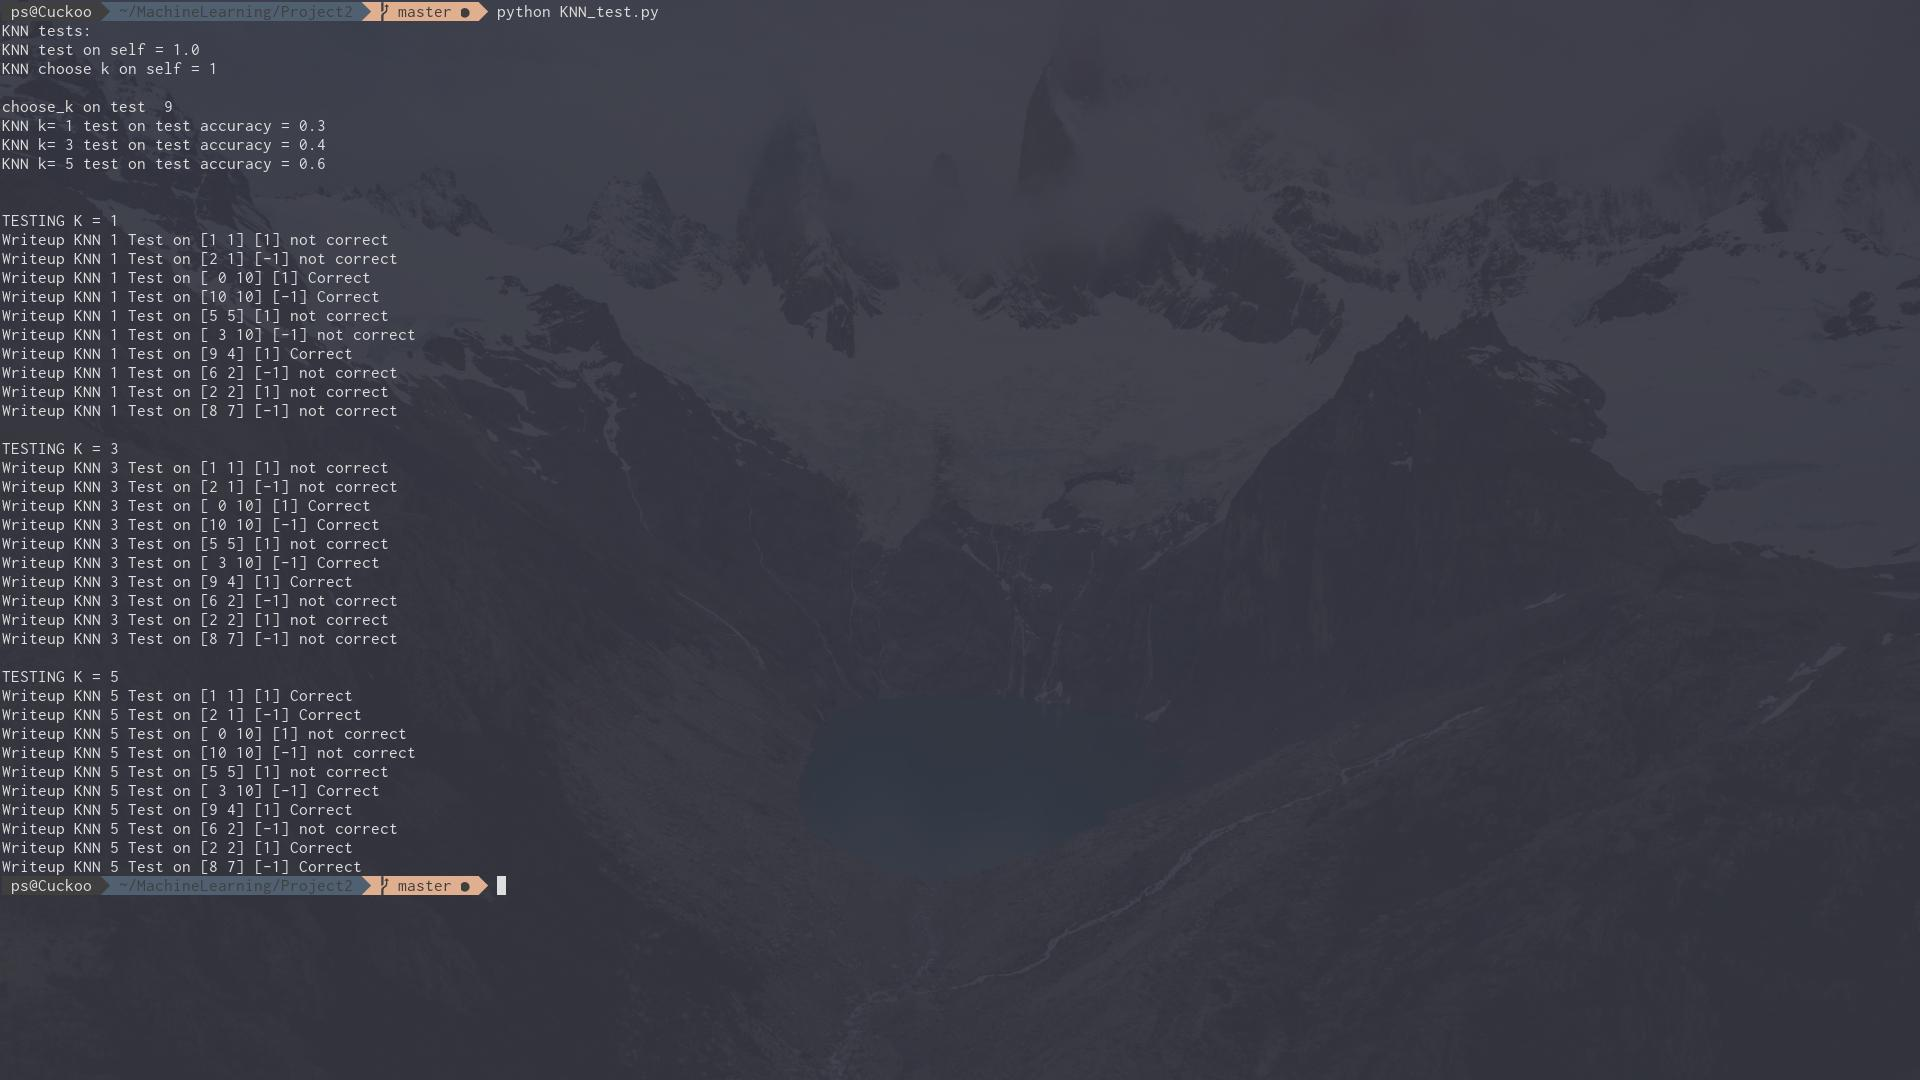
\includegraphics[scale=.24]{KNN.jpg}
	\footnote{The picture has a high resolution so you should be able to zoom in and see the detail, but the picure has also been included in the zip file so please refer to that if there is any issues}
	
\end{center}
	The best K for our Algorithm would be 9 with the accuracy of 0.7, for more details like which specific sample was predicted wrong refer to the picture below.
	\begin{center}
		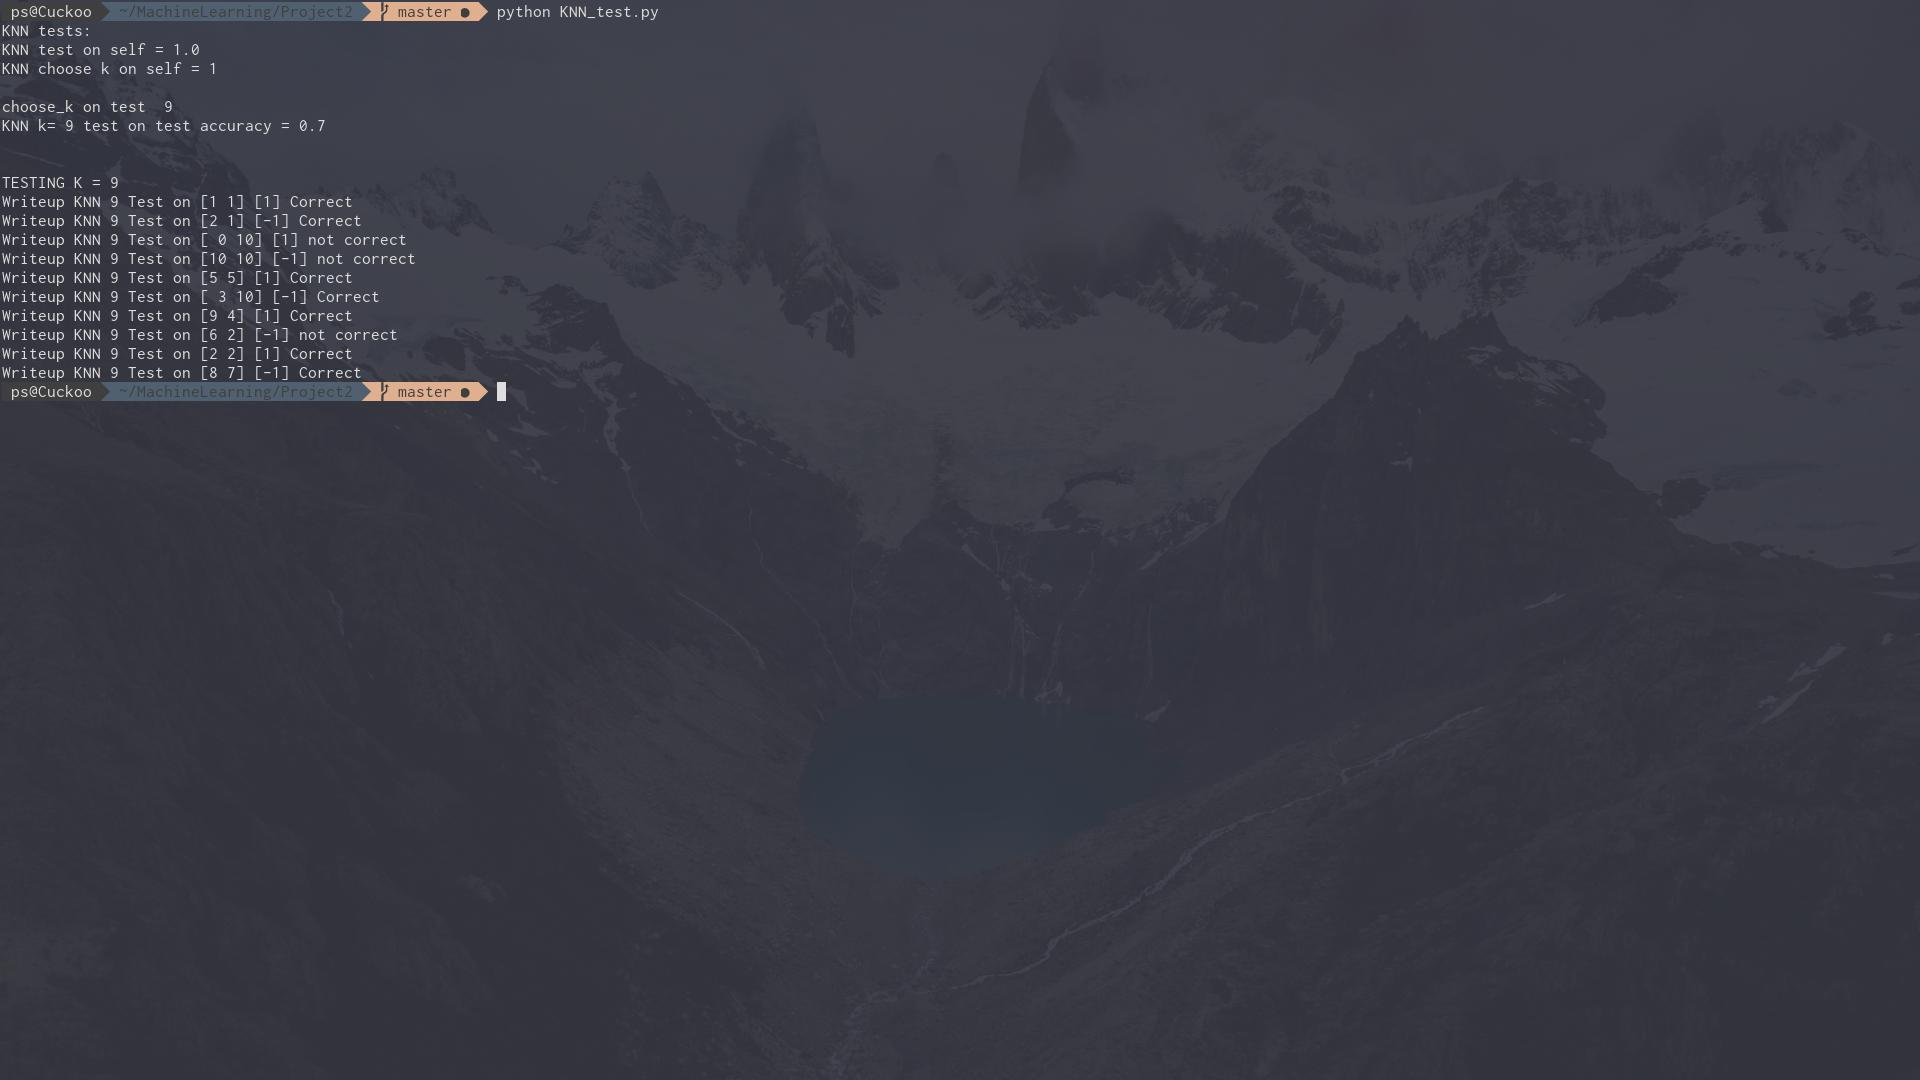
\includegraphics[scale=.24]{KNN2.jpg}
		\footnote{The picture has a high resolution so you should be able to zoom in and see the detail, but the picure has also been included in the zip file so please refer to that if there is any issues}
		
	\end{center}
	\section{KMeans Clustering}
	\subsection{Describe Implementation}
	
	\subsubsection{K\_Means}
	\subsubsection{K\_Means\_better}
	This function takes X, our sample data-set and the K value and runs the K-Mean algorithm 1000 times (can be changed by the user) we will then count the number of occurrences of each cluster center and return the ones with the most repeated or occurred cluster centers, this value will be stored in a numpy array of cluster centers and then returned.
	\begin{lstlisting}[language=Python]
	def K_Means_better(X, K):
	run = 1000
	bestCenterList = []
	occurences = []
	j = 0
	for i in range(run):
		try:
			result = K_Means(X, K)
			bestCenterList.append(result)
			j += 1
	except:
		pass
	for j in range(len(bestCenterList)):
		count = bestCenterList.count(bestCenterList[j])
		occurences.append(count)
	maxNum = 0
	for k in occurences:
		if (k > maxNum):
			maxNum = k
	return bestCenterList[maxNum]
	\end{lstlisting}
	\subsection{Algorithm Classification}
	\subsubsection{KMeans on K = 2, K = 3}
	The cluster centers have been labeled as a black dot. \\
	
	\begin{center}
		K = 2
		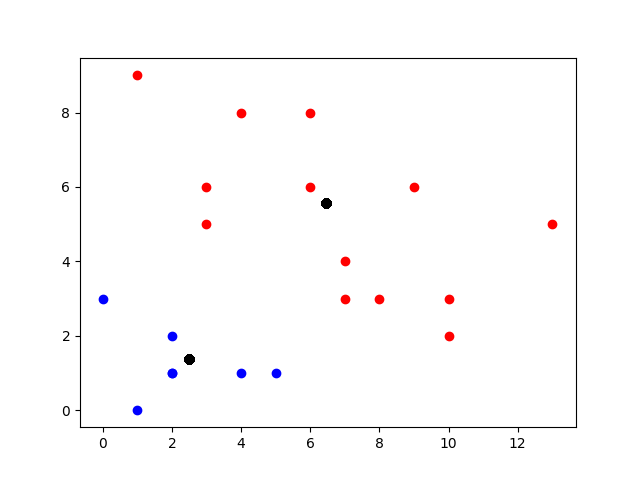
\includegraphics[scale=.8]{KMeans_K=2C.png}
	\end{center}
	\begin{center}
			K = 3
			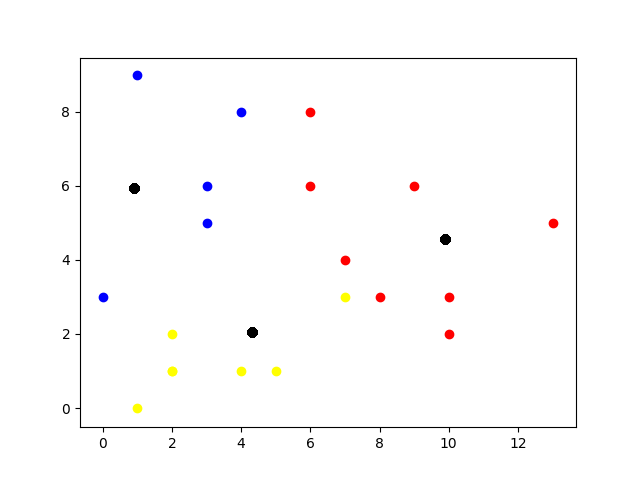
\includegraphics[scale=.8]{KMeans_K=3C.png}
	\end{center}
	
	\subsubsection{KMeans Better on K = 2, K = 3}
	\begin{center}
		K = 2
	\end{center}
	\begin{center}
		K = 3
	\end{center}
	
	\section{Perceptron}
	\subsection{Describe Implementation}
	\subsubsection{perceptron\_train}
	This function will be computing a weight (vector) and a bias using the data-set X and the labels for that set Y. We start with the initial weights and bias of 0 and we will kep track of epoch by a variable called epoch, we would also have to consider the fact that some data might not be linearly separable hence we will have another variable called maxEpoch which we would use to break our if the algorithm is not successful after maxEpoch tries. We will be using a while loop that checks if we are done yet, so we've gone an entire epoch without updating, or if we have reached the maxEpoch in which case the program gets out of the while loop and returns the weights and bias of the last iteration. Inside the while loop we are computing the activation and if the activation returns a number less than or equal to 0 we would ned to update hence we update our weight vector and the bias, they're both in the same list, the first element is weight vector, 2nd is bias(W\_B\_List) if data is linearly separable we would update our Done flag to true and get out of the loop and finally return the weight vector and bias (W\_B\_List)
	\begin{lstlisting}[language=Python]
	Done = False 
	epoch = 0 
	maxEpoch = 199
	activation = 0 
	W_B_List = [[],[]] 
	W_B_List[0] =[0]*len(X[0]) 
	W_B_List[1] = [0]
	while ( not Done or epoch < maxEpoch): 
		epoch+=1
		for i in range (len(X)):
			activation = 0
			for m in range(len(X[i])):
				activation += X[i][m] * W_B_List[0][m]
			activation+= W_B_List[1][0]
			if  (( activation * Y[i][0] ) <= 0):
				for j in range(len(X[0])):
					W_B_List[0][j] = W_B_List[0][j] + Y[i][0] * X[i][j]
				W_B_List[1][0] = W_B_List[1][0] + Y[i][0]
			else:
				Done = True 
	return W_B_List
	\end{lstlisting}
	
	\subsubsection{perceptron\_test}
	This function computes the accuracy of the weights and bias given the data-set X and their label Y. This function computes the activation for each of the samples in the data-set X and compares it with their label. If the activation matches the label we would increment our NumberOfCorrect variable at the end we will divide this number by the length of our data-set X to find the accuracy and we would return that number. 
	\begin{lstlisting}[language=Python]
	NumberOfCorrect = 0
	activation = 0
	for i, j in enumerate(X_test):
		activation = np.dot(j,w) + b 
		if activation * Y_test[i] > 0:
			NumberOfCorrect+=1
	return NumberOfCorrect/len(X_test)
	\end{lstlisting}
	 
	\subsection{Decision Boundary}
	I have used the Desmos website to plot the points and the decision boundary for this part. Blue points are the ones with label 1 and red points have label of -1. 
	The algorithms returns 2,4 for our weights and 2 for our bias hence we will be  using the function 
	$2X_1 + 4X_2 + 2 = 0$ we could simplify this function but since we will be drawing it to show the decision boundary there is no need.
	\begin{center}
		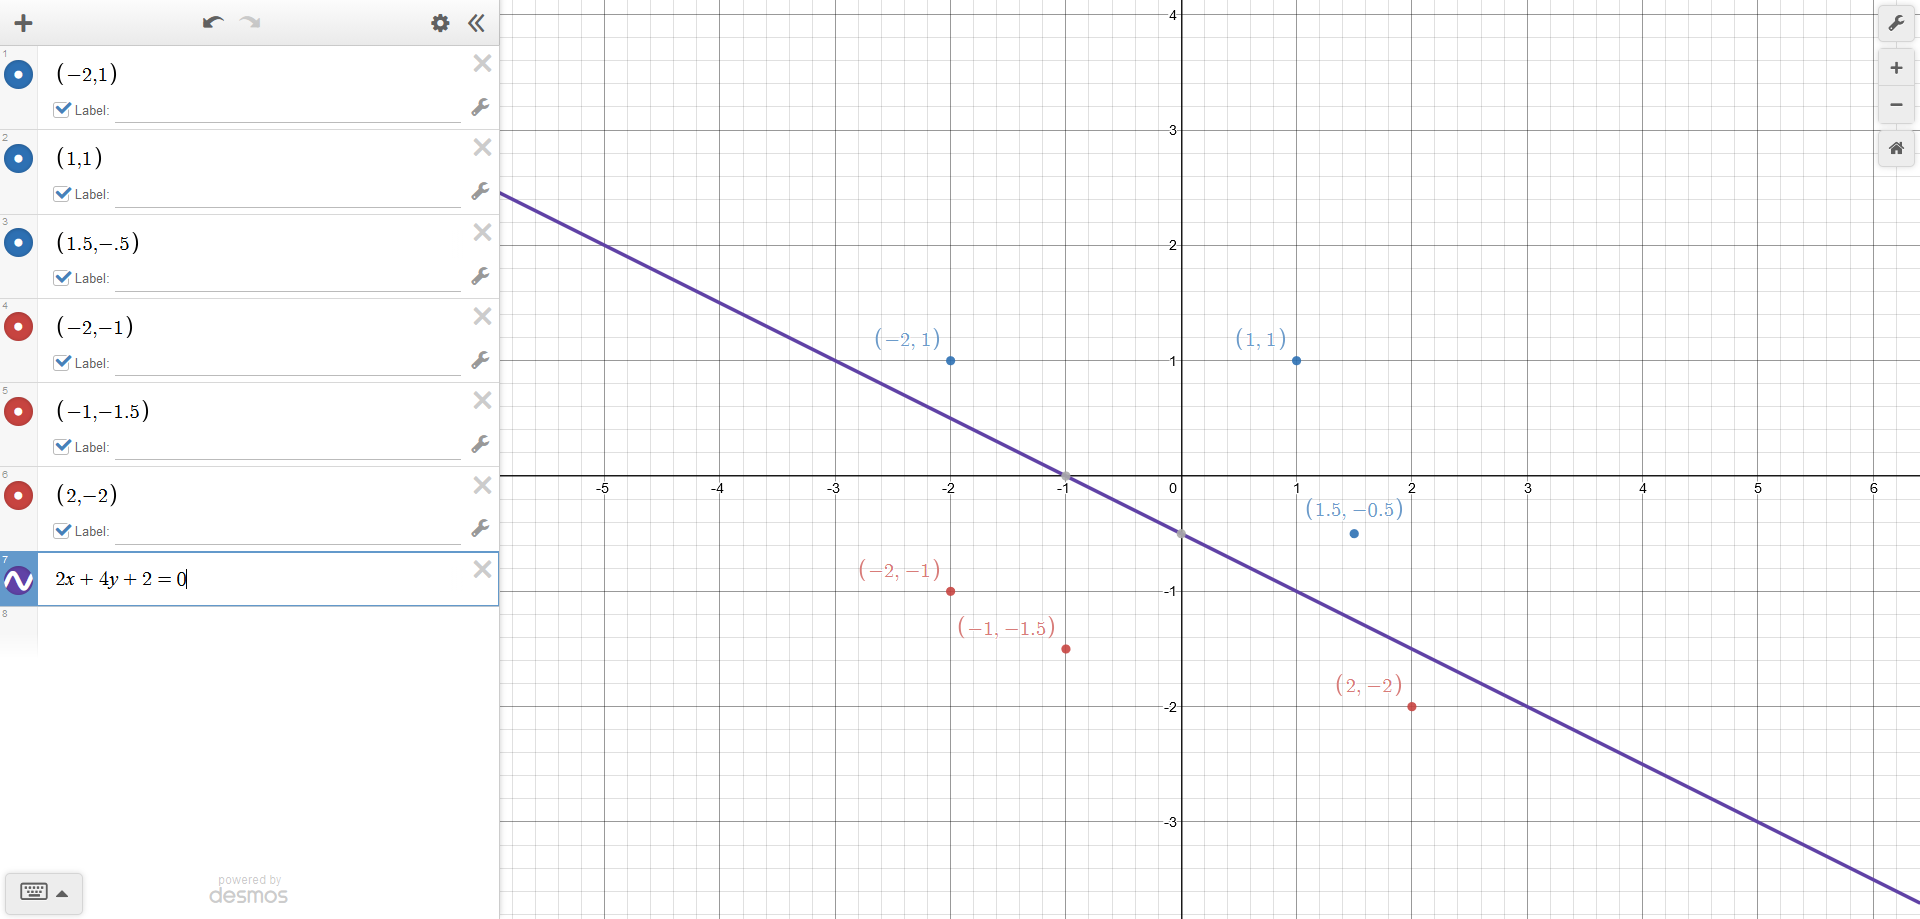
\includegraphics[scale=.24]{DB.png}
		\footnote{The picture has a high resolution so you should be able to zoom in and see the detail, but the picure has also been included in the zip file so please refer to that if there is any issues}
	\end{center}
	\begin{center}
	scaled larger for better visibility
	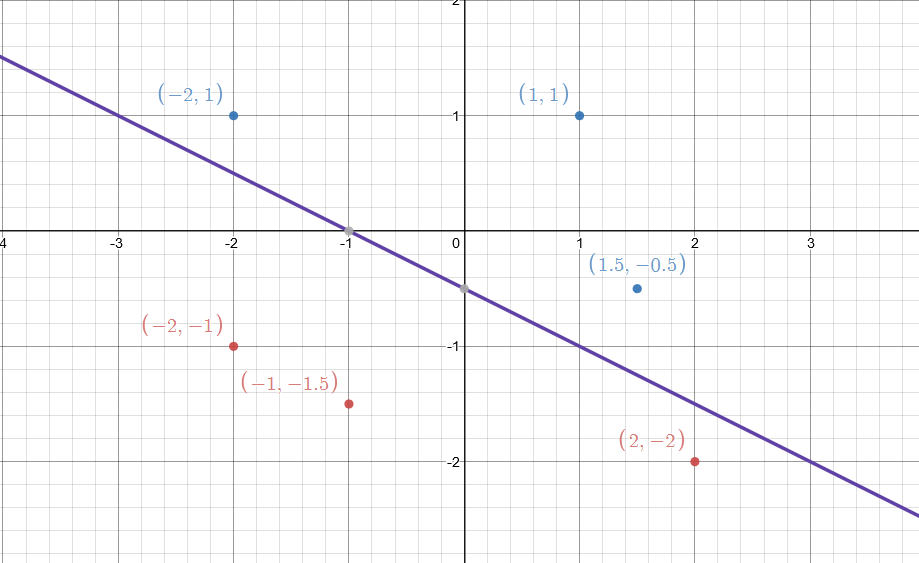
\includegraphics[scale=.65]{DB2.png}
\end{center}

\end{document}


